%%%%% this line is 80 chars wide, please don't make longer lines %%%%%%%%%%%%%%%
%mettre image, mais p-ê dans appendice
%montrer images 4 graphs en colonne
Let us speak now about the model of the peripheral auditory system from 
\cite{Model1, Model2, Model3} used to run experiments in this project. 

I will not go into the details of the model, but more on the use of it. 
You can see in \autoref{fig:modelsch} the schematic of the model.


%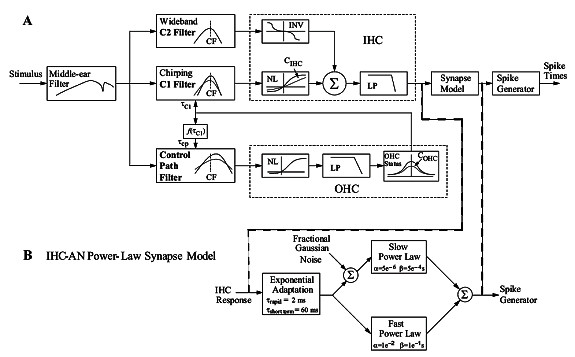
\includegraphics[width=0.45\textwidth]{images/www-bme-rochester-edu-schematicDiagram-level.jpg}

From the user point of view, the model consists of two main functions 
that are called "catmodel\_IHC" and "catmodel\_Synapse". Their prototype is

\texttt{vihc = catmodel\_IHC(pin, CF, nrep, tdres, reptime, cohc, cihc);}

and

\texttt{[synout, psth] = catmodel\_Synapse(vihc, CF, nrep, tdres, fibertype, implnt);}

like specified in the catmodel.m file of the model. 
Let us go deeper into what each parameters and return value of these functions mean.

The first function, \texttt{catmodel\_IHC}, takes as parameters 
a stimulus matrix (\texttt{pin}, in Pa), sampled at some sampling rate that is 
the inverse of \texttt{tdres}, the characteristic function (\texttt{CF}, in Hz) 
of the IHC for which we want to know the potential 
(\texttt{vihc}, in Volt) when stimulated. 
\texttt{reptime} is the time for one repetition of the stimulus, 
and \texttt{nrep} is the number of repetions we want to be run. 
\texttt{vihc} will contain the IHC potential for every repetition.
The \texttt{fibertype} parameter is used to tell the model which nerve fiber type
we "test" with the stimulus, distinguished by their spontaneus rate (SR) : 
low, medium or high (low : < 1 spike/s, medium : < 18 spike/s, high: 20-50 spike/s, 
according to \cite{AuditoryNeuroscience}). %82

The second function, \texttt{catmodel\_Synapse}, 
takes the IHC potential returned by \texttt{catmodel\_IHC}, 
with the same sampling rate, so the same \texttt{tdres}, which is also here the bin size
of the PSTH returned by the function (\texttt{psth}). 
The PSTH will be computed according to the specified number of repetitions (\texttt{nrep}).
The synapse output of the IHC (\texttt{synout}) is also returned by the function. 
The parameter \texttt{fibertype} means the same here as for \texttt{catmodel\_IHC}.
\texttt{cohc} and \texttt{cihc} represents the damages on respectively 
the outer hair cells and inner hair cells in the simulation, and, finally, 
\texttt{implnt} is used to indicate the precision we want in the simulation 
for some calculations in the model.

As an example of what result the model can give,
in \autoref{fig:g4tonestep} you can see some graphs that represents some signals of a 
simulation of a pure tone step stimulus. 

%\includegraphics[width=0.45\textwidth]{images/g4-tonestep-column.jpg} %do it !

%TODO
%\begin{figure}[h]
%	\centering
%	\includegraphics[width=0.45\textwidth]{images/images/g4-tonestep-column.jpg}
%	\caption{Example of model results (\cite{Model1})}
%	\label{fig:g4tonestep}
%\end{figure}

The first graph is a representation of one period of the stimulus. 
What was given to the model as \texttt{pin} was this, repeated %klé !!
times.
On the second graph, you can see the IHC potential from the first function
 in response of the last %%hgjsl !!
period of the stimulus (with dependencies on the preceding periods included).
The third graph shows you a part of the synapse output given by \texttt{catmodel\_Synapse}, 
for the same period as for the potential of IHC.
The fourth represents graph the periodogram for the entire stimulus, 
computed with help of the PSTH given by the second function.

%\begin{lstlisting}[caption={},captionpos=b]{}
%\end{lstlisting}

%\texttt{tdres} 

 





